\documentclass{article}
% 导言
\usepackage{xeCJK}
\usepackage{graphicx}
\usepackage{float}
% 正文区
\begin{document}
	% 标题
	\title{通信前言技术}
	\author{张兴锐}
	\date{}
%	\maketitle
	% 正文
	\section{LTE性能指标}
	\begin{enumerate}
		\item 数据峰值:上50M,下100M
		\item 延迟: 空闲转活跃100ms,用户面低于5ms
		\item 移动性:速率高达350km/h的用户设备链接
		\item 支持多种带宽分配
	\end{enumerate}
	\section{LTE网络体系架构}
	\subsection{LTE网络体系架构组成}
	\begin{enumerate}
		\item EPS :网络体系的全程
		\item E-UTRAN:演进UMTS陆地无线接入网络
		\item EPC: 演进分组核心网络
	\end{enumerate}
	\begin{figure}[H]
		\centering
		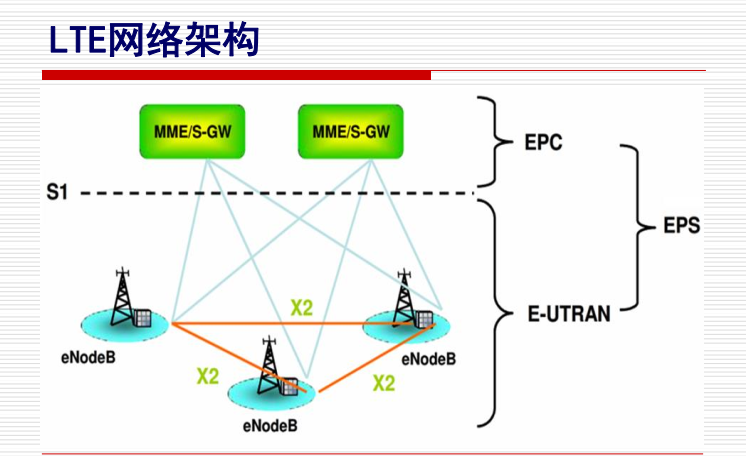
\includegraphics[width=0.7\linewidth]{LTE网络架构}
		\caption{LTE网络架构}
		\label{fig:lte}
	\end{figure}
	\subsection{LTE网络架构特点}
	\begin{enumerate}
		\item 网络结构更加简单扁平
		\item 取消RNC的集中控制,避免单点故障,有利于提高网络稳定性。
	\end{enumerate}
	\section{LTE关键技术}
	\subsection{多天线技术MIMO}
	\begin{description}
		\item[基本概念] 在发送和接收端采用多跟天线,多输入输出
		\item[采用MIMO的目的] 通过充分利用空间资源,提高频谱效率,增加系统容量,实现更广覆盖。
	\end{description}
	\subsubsection{单天线系统容量}
	\begin{figure}[H]
		\centering
		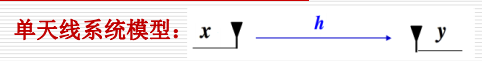
\includegraphics[width=0.7\linewidth]{单天线发射模型}
		\caption{单天线发射模型}
		\label{fig:}
	\end{figure}
	接收端:\(y = xh+n\)。\\
	假设发射段功率为$P_t$,则接收端功率为$|h|^2P_t$。
	接受信噪比$SNR = \frac{P_R}{\sigma^2}=\frac{|h|^2P_t}{\sigma^2}=|h|^2\rho$\\
	信道容量 $C_0 = Blog(1+SNR) = Blog(1+||h|^2\rho)$ \\
	单位频谱信道容量:$C = log(1+|h|^2\rho)$	\\
	\subsubsection{各类系统容量}
	\begin{description}
		\item[SISO] $C = log(1+|h|^2\rho)$
		\item[SIMO] $C = log(1+\sum_{i = 1}^{M}|h|^2\rho)$
		\item[MISI] $C = \frac{1}{N}log(1+\sum_{i = 1}^{N}|h|^2\rho)$
		\item[MIMO] $C = log[det(I_M+\frac{\rho}{N}HH^{*})]$
	\end{description}
	\textbf{在MIMO系统中,如果N,M足够大,$C = min\{N,M\}log(\rho/2)$},其系统容量随着天线数目的增加而线性增加
	\subsection{正交频分复用(OFDM)技术}
	\subsubsection{OFMD实现流程}
	\begin{figure}[H]
		\centering
		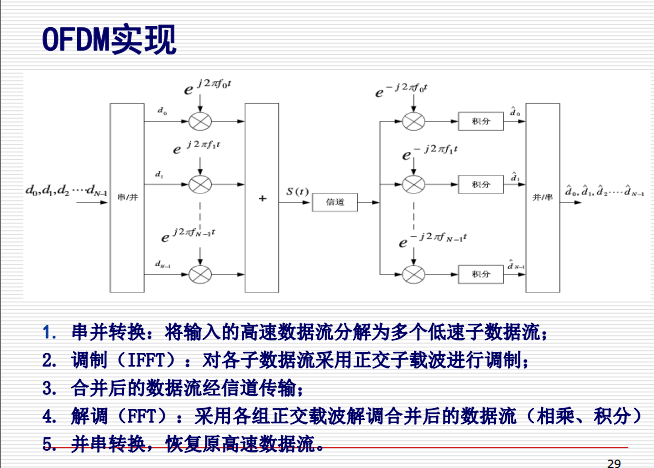
\includegraphics[width=\linewidth]{OFDM实现流程}
		\caption{OFDM实现流程}
		\label{fig:ofdm}
	\end{figure}
	\subsubsection{OFMD的优缺点}
	\begin{description}
		\item[优点] 高频率效率;对抗频率选择性衰落;支持快带传输,消除ISIS影响。
		\item[缺点] 对频率偏移和相位噪声很敏感;峰均比(PAPR)较大,导致射频放大器的功效较低。
	\end{description}
\end{document}